\section*{問題4}
\begin{enumerate}
    \renewcommand{\labelenumi}{\Alph{enumi}.}
    \item (B)で示す.
    \item
    $\hat{c}_1$, $\hat{c}_{\rm rand}$, $\hat{c}_{\rm min}$の3種類のコインにおいて,$\bm{{\rm P}}\{|\hat{c}-\bm{{\rm E}}c|>\varepsilon\}$を近似し,$\varepsilon$の関数としてそのグラフを描くと,以下の図のようになる.
    尚,同じプロットにおいて,Hoeffdingの上界($2e^{-2\varepsilon^2n}$)をオレンジの線で表している.
    \begin{figure}[H]
        \begin{center}
            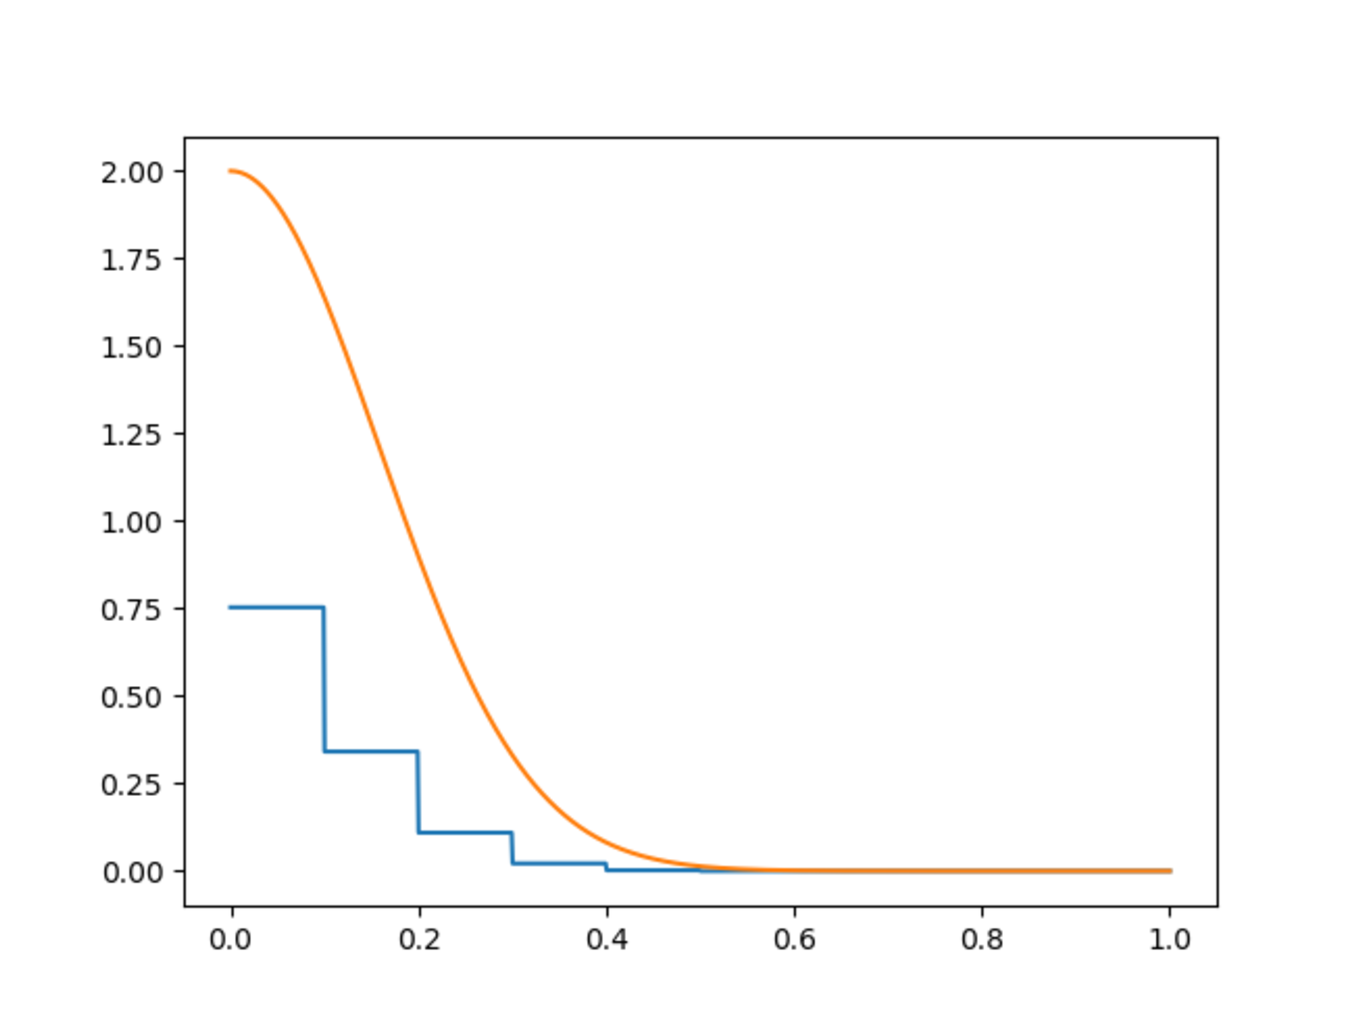
\includegraphics[width=100mm]{./figures/section_4/Hoeffding_c1.eps}
            \captionsetup{labelformat=empty,labelsep=none}
            \caption{$\hat{c}_1$}
        \end{center}
    \end{figure}
    \begin{figure}[H]
        \begin{center}
            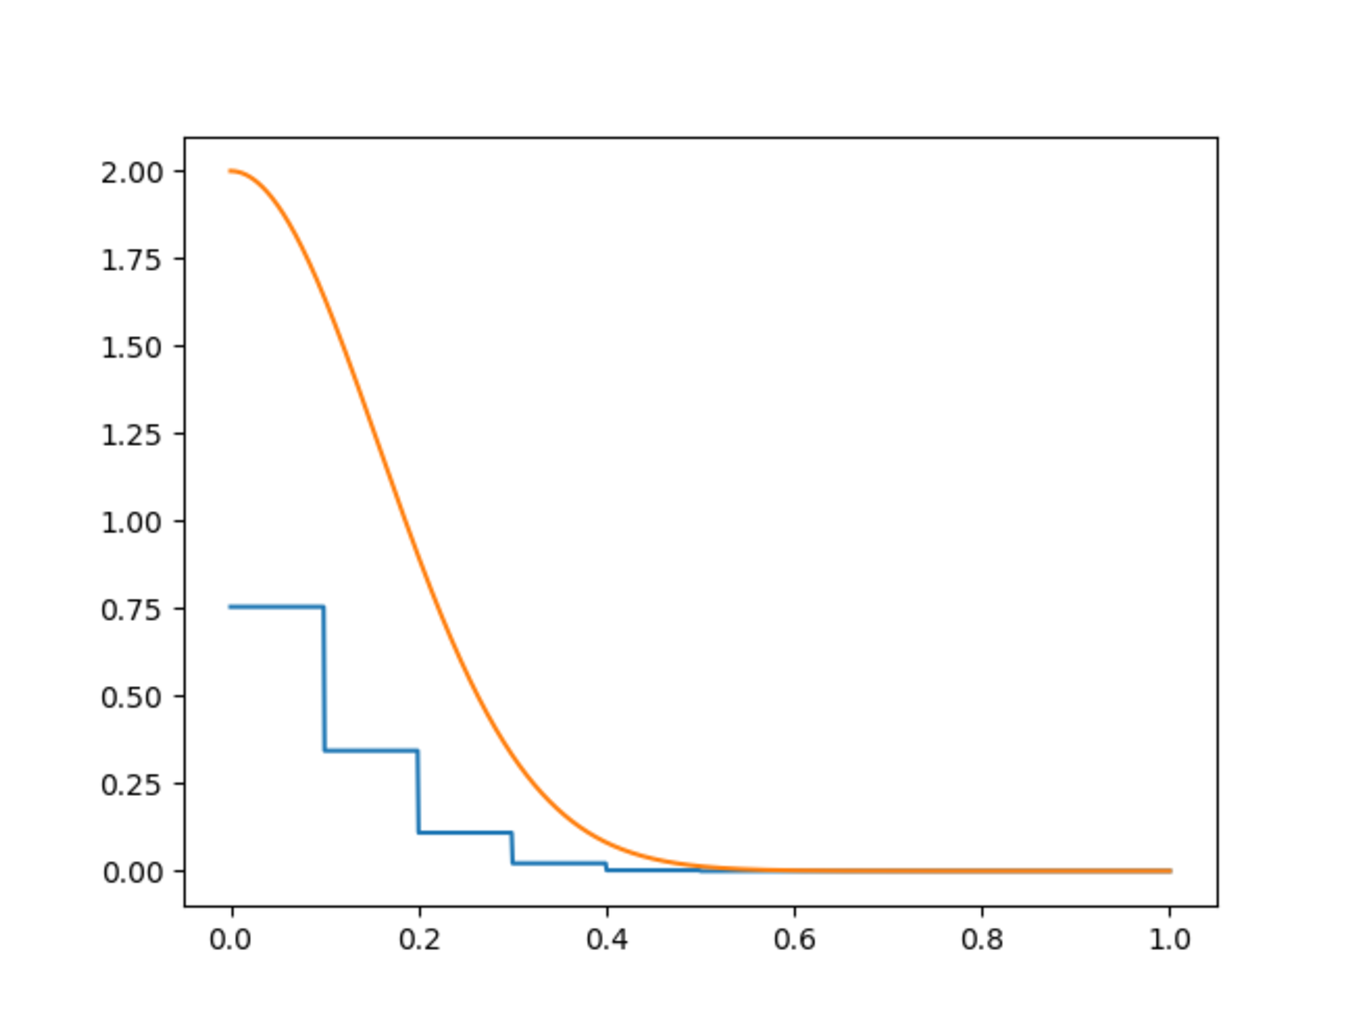
\includegraphics[width=100mm]{./figures/section_4/Hoeffding_crand.eps}
            \captionsetup{labelformat=empty,labelsep=none}
            \caption{$\hat{c}_{\rm rand}$}
        \end{center}
    \end{figure}
    \begin{figure}[H]
        \begin{center}
            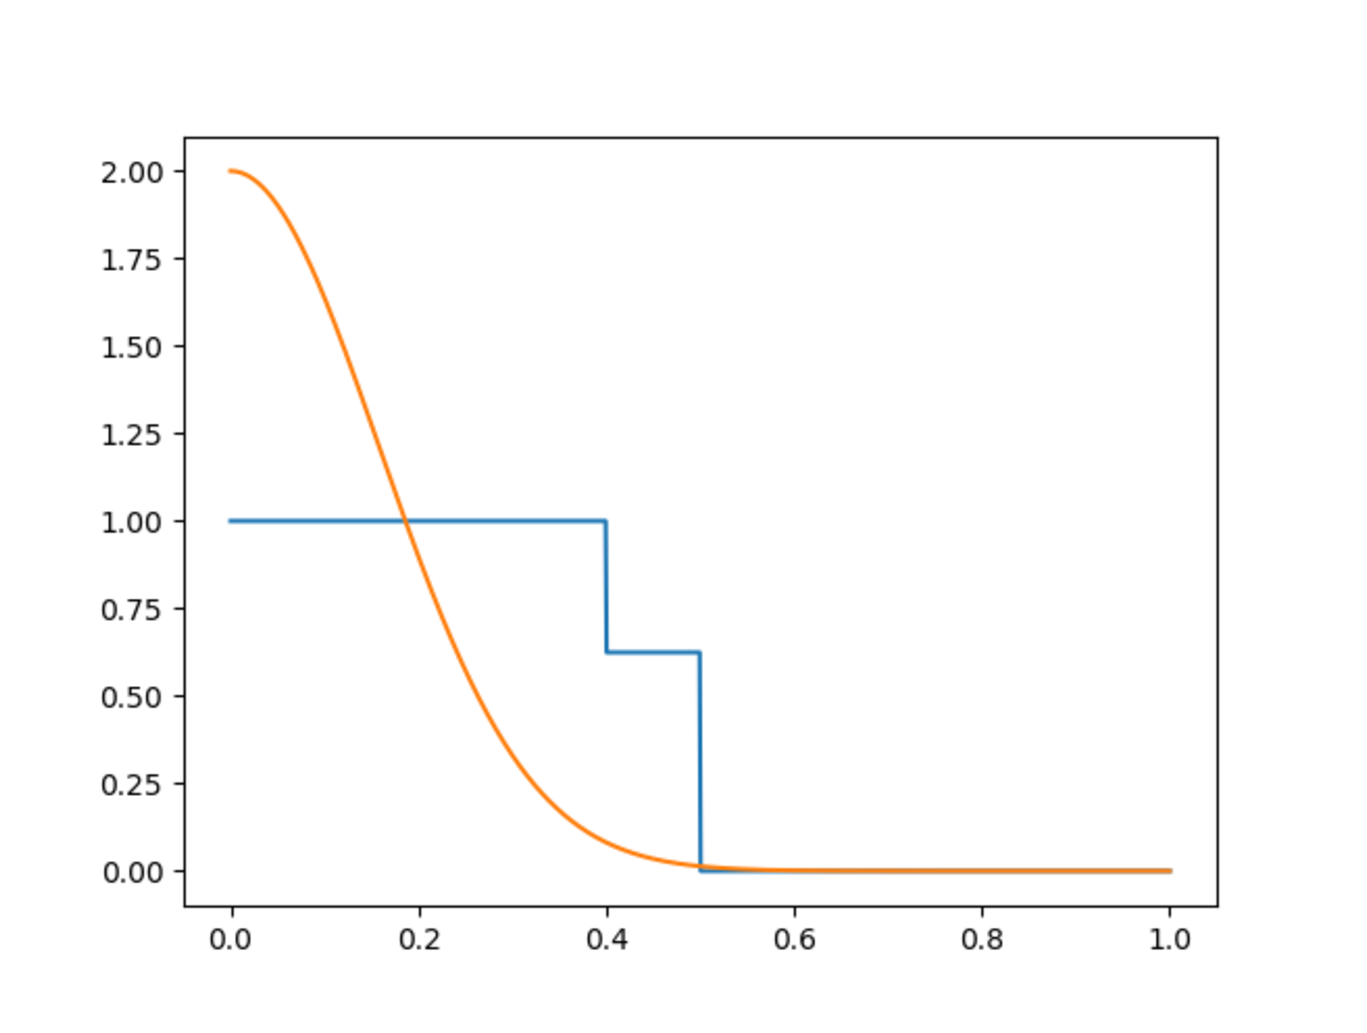
\includegraphics[width=100mm]{./figures/section_4/Hoeffding_cmin.eps}
            \captionsetup{labelformat=empty,labelsep=none}
            \caption{$\hat{c}_{\rm min}$}
        \end{center}
    \end{figure}
    \item
    $c_1$と$c_{\rm rand}$はHoeffdingの不等式に従うが,$c_{\rm min}$は従わない.
    これは,$c_{\rm min}$が1000枚のコインの中の任意のコインではなく,表の数が最も少なかった特定のコインであるからである.
\end{enumerate}